\subsubsection{Förderband}
Da die Schwungräder durch den Abwurf abgebremst werden, müssen Sie nach jedem Wurf erneut auf die gewünschte Drehzahl beschleunigt werden. Deshalb hat die Zuführung der Bälle in Abständen zu erfolgen. Weiter müssen die einzelnen Tennisbälle immer mit der gleichen Geschwindigkeit bei den Schwungrädern eintreffen, damit eine konstante Wurfweite entsteht. Die beste Art, beides zusammen zu realisieren ist ein Förderband. Das Förderband wird zwischen den zwei Acrylglasplatten aufgespannt. Der Antrieb des Förderbandes erfolgt mit einem DC-Motor. Dieser wird mit einem Verhältnis von !!i=5:1 übersetzt, um das benötigte Drehmoment an die Antriebstrommel von !!Nm zu übertragen. Die Berechnungen dazu sind im entsprechenden Kapitel ersichtlich. Auf dem Förderband, welches aus einem Zahnriemen besteht, sind konkave Führungsblätter angebracht. Diese sind so aus-gerundet, damit der Ball möglichst lange geführt werden kann und die Führungsblätter nicht in Berührung der Schwungräder kommen. Die Führungsblätter werden voraussichtlich mit dem Förderband verschweisst.
\begin{figure}
	\centering
	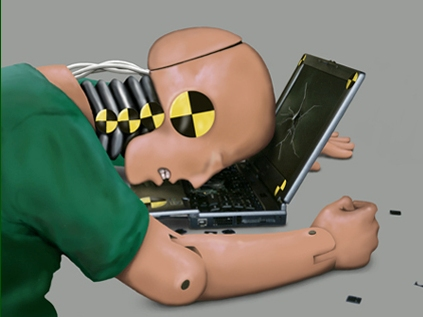
\includegraphics[width=0.9\textwidth]{Enddokumentation/CrashTestDummy.jpg}
	\caption{Grafik Förderband}
	\label{fig:Grafik Förderband}	
\end{figure}
Aus Testversuchen der Ballzuführung wurde erkannt, dass für einen idealen Abwurf beide Räder zeitgleich den Ball einklemmen müssen. Somit müssen die Bälle zunächst unterhalb des oberen Schwungrades gefördert und anschliessend in einem $45^\cdot$ Winkel nach oben zugeführt werden. Dazu dient ein Führungselement. Inwiefern dieses aussieht ist noch völ-lig offen. Als Ideen stehen zwei Stangen oder ein Blech zur Auswahl. Für den Riemen hat dies zur Folge, dass hohe Schaufeln den Ball führen müssen. Die folgende Grafik zeigt eine Auswahl möglicher Ausführungen der Schaufeln am Band.
\begin{figure}
	\centering
	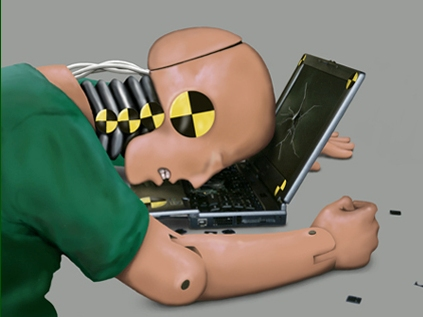
\includegraphics[width=0.9\textwidth]{Enddokumentation/CrashTestDummy.jpg}
	\caption{Grafiken (Schaufel genietet, geklebt, nur Klebauftrag)}
	\label{fig:Grafiken (Schaufel genietet, geklebt, nur Klebauftrag)}	
\end{figure}

Die Anforderung an die Ballnachführungsantrieb sind nicht hoch. Es sind das Gewicht und die Zugkraft von !!Berechnung!!. Da die Kraft gering ist, kann dieser Antrieb mittels eines DC-Motors realisiert werden. Dieser kann mittels eines PWM-Signals über einen entsprechenden Transistor gesteuert werden. Die Abbildung \ref{fig:Schema_DC-Motor} zeigt, wie Ansteuerung des DC-Motors umgesetzt werden wird.
	\begin{figure}[h!] %{0.45\textwidth}
		\centering
		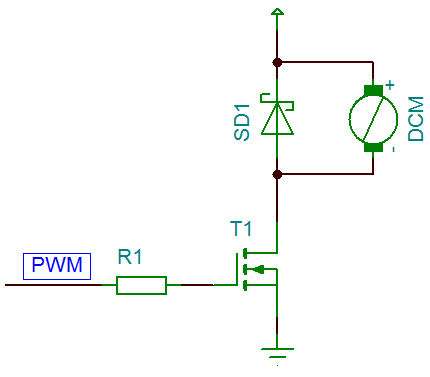
\includegraphics[width=0.3\textwidth]{Enddokumentation/Loesungskonzept/Bilder/SchemaDcMotor.png}
		\caption{Schema der DC-Motoransteuerung}
		\label{fig:Schema_DC-Motor}
	\end{figure}